\section{Introduction}
%%%%%%%%%%%% MID WAY AGENDA %%%%%%%%%%%%%%
% \begin{frame}<beamer>
% \frametitle{Daniel Bähner Andersen}
% \tableofcontents[currentsection]
% \end{frame}	
%%%%%%%%%%%% MID WAY AGENDA %%%%%%%%%%%%%%

\begin{frame}{Introduction}{}
    \begin{itemize}            
	\item<1-> Water distribution network
	    \begin{itemize}  
			\item<1-> Necessary infrastructure 
			\item<1-> High energy consumption 
		\end{itemize}   
\end{itemize}
\begin{itemize}	
	\item<2-> Possible solution 
	\begin{itemize}	
		\item<2-> Introduction of water tower
		\item<2-> Advance control that ensure satisfying performance
	\end{itemize}
\end{itemize}
\begin{itemize}	
		\item<3-> \textit{How can a water tower be implemented in a water distribution network and controlled to minimize the cost of running the distribution network without violating constraints and compromising the water quality.}
    \end{itemize}           
\end{frame}



\begin{frame}{System description}{System description}

\begin{itemize}            
	\item<1-> 1:20 downscaled version of real water distribution system
\end{itemize} 
\vspace{-0.5cm}
\begin{figure}[H]
	\centering
	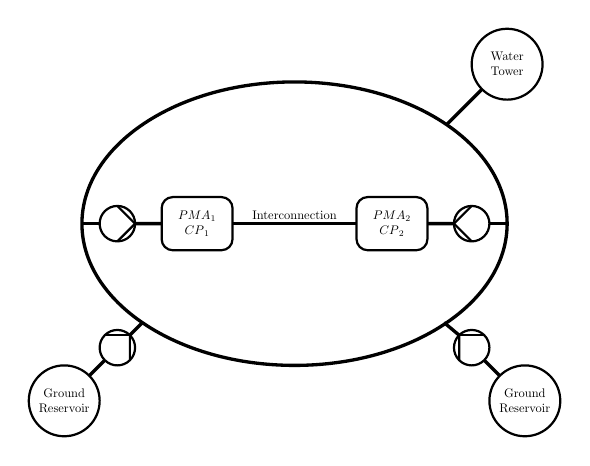
\begin{tikzpicture}[scale=0.45,transform shape]
\tikzstyle{box} = [draw,thick,rounded corners, minimum height=15mm, minimum width=20mm, align=center, text centered]
%Main Ring
\draw[very thick] (7,5.5) ellipse (6 and 4);
%Pump
\draw[thick,transform shape] (2,5.5) circle (0.5);
\draw[thick,transform shape] (2.5,5.5) -- (2,6);
\draw[thick,transform shape] (2.5,5.5) -- (2,5);
%Pump
\begin{scope} [rotate around={180:(12,5.5)}]
\draw[thick,transform shape] (12,5.5) circle (0.5);
\draw[thick,transform shape] (12.5,5.5) -- (12,6);
\draw[thick,transform shape] (12.5,5.5) -- (12,5);
\end{scope}
%Pump
\begin{scope} [rotate around={135:(12,2)}]
\draw[thick,transform shape] (12,2) circle (0.5);
\draw[thick,transform shape] (12.5,2) -- (12,2.5);
\draw[thick,transform shape] (12.5,2) -- (12,1.5);
\end{scope}
%Pump
\begin{scope} [rotate around={45:(2,2)}]
\draw[thick,transform shape] (2,2) circle (0.5);
\draw[thick,transform shape] (2.5,2) -- (2,2.5);
\draw[thick,transform shape] (2.5,2) -- (2,1.5);
\end{scope}
%Reservoirs
\node[thick,draw,circle,minimum width=20mm,align=center] (R1) at (0.5,0.5) {Ground \\ Reservoir};
\node[thick,draw,circle,minimum width=20mm,align=center] (ER1) at (13,10) {Water \\ Tower};
\node[thick,draw,circle,minimum width=20mm,align=center] (R2) at (13.5,0.5) {Ground \\ Reservoir};
%PMA and interconnection
\node[box] (PMA1) at (4.25,5.5) {$\text{PMA}_1$ \\ $\text{CP}_1$};
\node[box] (PMA2) at (9.75,5.5) {$\text{PMA}_2$ \\ $\text{CP}_2$};
\draw[very thick](PMA1) -- (PMA2);
\node[align=center] (PMAc) at (7,5.75) {Interconnection};
%Connections
\draw[very thick](1.2,1.2) -- (1.65,1.65);
\draw[very thick](2.34,2.34) -- (2.71,2.71);
\draw[very thick](12.8,1.2) -- (12.36,1.64);
\draw[very thick](11.66,2.34) -- (11.22,2.71);
\draw[very thick](13,5.5) -- (12.5,5.5);
\draw[very thick](11.5,5.5) -- (PMA2);
\draw[very thick](1,5.5) -- (1.5,5.5);
\draw[very thick](2.5,5.5) -- (PMA1);
\draw[very thick](12.28,9.28) -- (11.29,8.29);
\end{tikzpicture} 
\end{figure}\vspace{-0.5cm}
\end{frame}


\begin{frame}{System description}{System description}
\begin{figure}[H]
\centering
\resizebox{1\linewidth}{!}{\tikzset{pressure/.style={draw, circle, inner sep=0pt, text width=5mm, align=center}}
\tikzset{difpres/.style={draw, circle, inner sep=0pt, text width=6mm, align=center}}
\tikzset{connect/.style={draw,circle, inner sep=0pt, text width=2mm, align=center,fill=black}}
\tikzset{evalve/.style={draw, circle, inner sep=0pt, text width=3mm, align=center}}
\begin{tikzpicture}



%Pump north
\node[draw,circle,minimum size=1cm] (p0) at (6,6) {};
\node(p1) at ($(p0)+(-0.5,0)$) {};
\node(p2) at ($(p1)+(0.5,0.5)$) {};
\node(p3) at ($(p1)+(1,0)$) {};
\draw(p1.center) -- (p2.center) -- (p3.center);
\node at ($(p1)+(1.5,0)$) {\Large $C_{18}$};

%Pump north
\node[draw,circle,minimum size=1cm] (p0) at (-5,9) {};
\node(p1) at ($(p0)+(-0.5,0)$) {};
\node(p2) at ($(p1)+(0.5,0.5)$) {};
\node(p3) at ($(p1)+(1,0)$) {};
\draw(p1.center) -- (p2.center) -- (p3.center);
\node at ($(p1)+(1.5,0)$) {\Large $C_{32}$};

%Pump north
\node[draw,circle,minimum size=1cm] (p0) at (20,6) {};
\node(p1) at ($(p0)+(-0.5,0)$) {};
\node(p2) at ($(p1)+(0.5,0.5)$) {};
\node(p3) at ($(p1)+(1,0)$) {};
\draw(p1.center) -- (p2.center) -- (p3.center);
\node at ($(p1)+(1.5,0)$) {\Large $C_{25}$};

%Pump north
\node[draw,circle,minimum size=1cm] (p0) at (-1.5,0.5) {};
\node(p1) at ($(p0)+(-0.5,0)$) {};
\node(p2) at ($(p1)+(0.5,0.5)$) {};
\node(p3) at ($(p1)+(1,0)$) {};
\draw(p1.center) -- (p2.center) -- (p3.center);
\node at ($(p1)+(1.5,0)$) {\Large $C_{2}$};

%Pump north
\node[draw,circle,minimum size=1cm] (p0) at (28,0.5) {};
\node(p1) at ($(p0)+(-0.5,0)$) {};
\node(p2) at ($(p1)+(0.5,0.5)$) {};
\node(p3) at ($(p1)+(1,0)$) {};
\draw(p1.center) -- (p2.center) -- (p3.center);
\node at ($(p1)+(1.5,0)$) {\Large $C_{16}$};

%man-valve
\node(n1) at (6.25,5) {};
\draw(n1.center) -- ($(n1)-(0.5,0)$) --
($(n1)-(0,1)$) -- ($(n1)-(0.5,1)$) --  (n1.center);
\draw($(n1)-(0.75,0.25)$) -- ($(n1)-(0.75,0.75)$) -- 
($(n1)-(0.75,0.5)$) --  ($(n1)-(0.25,0.5)$);
%\node at ($(n1)+(0.5,-0.5)$) {\Large $C_{18d}$};

%man-valve
\node(n1) at (6.25,8) {};
\draw(n1.center) -- ($(n1)-(0.5,0)$) --
($(n1)-(0,1)$) -- ($(n1)-(0.5,1)$) --  (n1.center);
\draw($(n1)-(0.75,0.25)$) -- ($(n1)-(0.75,0.75)$) -- 
($(n1)-(0.75,0.5)$) --  ($(n1)-(0.25,0.5)$);
%\node at ($(n1)+(0.5,-0.5)$) {\Large $C_{18u}$};

%man-valve
\node(n1) at (20.25,8) {};
\draw(n1.center) -- ($(n1)-(0.5,0)$) --
($(n1)-(0,1)$) -- ($(n1)-(0.5,1)$) --  (n1.center);
\draw($(n1)-(0.75,0.25)$) -- ($(n1)-(0.75,0.75)$) -- 
($(n1)-(0.75,0.5)$) --  ($(n1)-(0.25,0.5)$);
%\node at ($(n1)+(0.5,-0.5)$) {\Large $C_{25u}$};

%man-valve
\node(n1) at (20.25,5) {};
\draw(n1.center) -- ($(n1)-(0.5,0)$) --
($(n1)-(0,1)$) -- ($(n1)-(0.5,1)$) --  (n1.center);
\draw($(n1)-(0.75,0.25)$) -- ($(n1)-(0.75,0.75)$) -- 
($(n1)-(0.75,0.5)$) --  ($(n1)-(0.25,0.5)$);
%\node at ($(n1)+(0.5,-0.5)$) {\Large $C_{25d}$};

%man-valve
\node(n1) at (-1.25,2.5) {};
\draw(n1.center) -- ($(n1)-(0.5,0)$) --
($(n1)-(0,1)$) -- ($(n1)-(0.5,1)$) --  (n1.center);
\draw($(n1)-(0.75,0.25)$) -- ($(n1)-(0.75,0.75)$) -- 
($(n1)-(0.75,0.5)$) --  ($(n1)-(0.25,0.5)$);
%\node at ($(n1)+(0.4,-0.5)$) {\Large $C_{3}$};

%man-valve
\node(n1) at (-1.25,-0.5) {};
\draw(n1.center) -- ($(n1)-(0.5,0)$) --
($(n1)-(0,1)$) -- ($(n1)-(0.5,1)$) --  (n1.center);
\draw($(n1)-(0.75,0.25)$) -- ($(n1)-(0.75,0.75)$) -- 
($(n1)-(0.75,0.5)$) --  ($(n1)-(0.25,0.5)$);
%\node at ($(n1)+(0.4,-0.5)$) {\Large $C_{1}$};

%man-valve
\node(n1) at (-4.75,11.5) {};
\draw(n1.center) -- ($(n1)-(0.5,0)$) --
($(n1)-(0,1)$) -- ($(n1)-(0.5,1)$) --  (n1.center);
\draw($(n1)-(0.75,0.25)$) -- ($(n1)-(0.75,0.75)$) -- 
($(n1)-(0.75,0.5)$) --  ($(n1)-(0.25,0.5)$);
%\node at ($(n1)+(0.5,-0.5)$) {\Large $C_{6}$};

%man-valve
\node(n1) at (-4.75,7.5) {};
\draw(n1.center) -- ($(n1)-(0.5,0)$) --
($(n1)-(0,1)$) -- ($(n1)-(0.5,1)$) --  (n1.center);
\draw($(n1)-(0.75,0.25)$) -- ($(n1)-(0.75,0.75)$) -- 
($(n1)-(0.75,0.5)$) --  ($(n1)-(0.25,0.5)$);
%\node at ($(n1)+(0.5,-0.5)$) {\Large $C_{5}$};

%man-valve
\node(n1) at (28.25,-0.5) {};
\draw(n1.center) -- ($(n1)-(0.5,0)$) --
($(n1)-(0,1)$) -- ($(n1)-(0.5,1)$) --  (n1.center);
\draw($(n1)-(0.75,0.25)$) -- ($(n1)-(0.75,0.75)$) -- 
($(n1)-(0.75,0.5)$) --  ($(n1)-(0.25,0.5)$);
%\node at ($(n1)+(0.5,-0.5)$) {\Large $C_{17}$};

%man-valve
\node(n1) at (28.25,2.5) {};
\draw(n1.center) -- ($(n1)-(0.5,0)$) --
($(n1)-(0,1)$) -- ($(n1)-(0.5,1)$) --  (n1.center);
\draw($(n1)-(0.75,0.25)$) -- ($(n1)-(0.75,0.75)$) -- 
($(n1)-(0.75,0.5)$) --  ($(n1)-(0.25,0.5)$);
%\node at ($(n1)+(0.5,-0.5)$) {\Large $C_{15}$};

%elec-valve
\node(n1) at (10.25,11.5) {};
\draw(n1.center) -- ($(n1)-(0.5,0)$) --
($(n1)-(0,1)$) -- ($(n1)-(0.5,1)$) --  (n1.center);
\draw($(n1)-(0.75,0.5)$) circle (1.5mm); 
\draw($(n1)-(0.6,0.5)$)--  ($(n1)-(0.25,0.5)$);
\node at ($(n1)+(0.3,-0.5)$) {\Large $C_{24}$};

%elec-valve
\node(n1) at (-1.25,11.5) {};
\draw(n1.center) -- ($(n1)-(0.5,0)$) --
($(n1)-(0,1)$) -- ($(n1)-(0.5,1)$) --  (n1.center);
\draw($(n1)-(0.75,0.5)$) circle (1.5mm); 
\draw($(n1)-(0.6,0.5)$)--  ($(n1)-(0.25,0.5)$);
\node at ($(n1)+(0.3,-0.5)$) {\Large $C_{20}$};

%elec-valve
\node(n1) at (24.25,11.5) {};
\draw(n1.center) -- ($(n1)-(0.5,0)$) --
($(n1)-(0,1)$) -- ($(n1)-(0.5,1)$) --  (n1.center);
\draw($(n1)-(0.75,0.5)$) circle (1.5mm); 
\draw($(n1)-(0.6,0.5)$)--  ($(n1)-(0.25,0.5)$);
\node at ($(n1)+(0.3,-0.5)$) {\Large $C_{31}$};

%elec-valve
\node(n1) at (13.25,11.5) {};
\draw(n1.center) -- ($(n1)-(0.5,0)$) --
($(n1)-(0,1)$) -- ($(n1)-(0.5,1)$) --  (n1.center);
\draw($(n1)-(0.75,0.5)$) circle (1.5mm); 
\draw($(n1)-(0.6,0.5)$)--  ($(n1)-(0.25,0.5)$);
\node at ($(n1)+(0.3,-0.5)$) {\Large $C_{27}$};

%man-valve
%\draw[very thick](-0.25,-1) -- (0.25,-1) -- (-0.25,-2) -- (0.25,-2) -- (-0.25,-1) -- (0.25,-1);
%\draw[very thick](0,-1.5) -- (-0.5,-1.5);
%\draw[very thick](-0.5,-1.25) -- (-0.5,-1.75);


%GND
\node(g1) at (-1.5,-2.5) {};
\draw(g1.center) -- ($(g1)+(0.3,0)$) -- ($(g1)-(0.3,0)$);
\draw($(g1)-(0.15,0.1)$) -- ($(g1)+(0.15,-0.1)$);

%GND
\node(g1) at (-1.5,9.5) {};
\draw(g1.center) -- ($(g1)+(0.3,0)$) -- ($(g1)-(0.3,0)$);
\draw($(g1)-(0.15,0.1)$) -- ($(g1)+(0.15,-0.1)$);

%GND
\node(g1) at (28,-2.5) {};
\draw(g1.center) -- ($(g1)+(0.3,0)$) -- ($(g1)-(0.3,0)$);
\draw($(g1)-(0.15,0.1)$) -- ($(g1)+(0.15,-0.1)$);

%GND
\node(g1) at (13,9.5) {};
\draw(g1.center) -- ($(g1)+(0.3,0)$) -- ($(g1)-(0.3,0)$);
\draw($(g1)-(0.15,0.1)$) -- ($(g1)+(0.15,-0.1)$);

%GND
\node(g1) at (24,9.5) {};
\draw(g1.center) -- ($(g1)+(0.3,0)$) -- ($(g1)-(0.3,0)$);
\draw($(g1)-(0.15,0.1)$) -- ($(g1)+(0.15,-0.1)$);

%GND
\node(g1) at (10,9.5) {};
\draw(g1.center) -- ($(g1)+(0.3,0)$) -- ($(g1)-(0.3,0)$);
\draw($(g1)-(0.15,0.1)$) -- ($(g1)+(0.15,-0.1)$);


%pipe
\node(r1) at (12,3) {};
\draw (r1.center) -- ($(r1)+(1.5,0)$) arc (90:-90:0.05) -- 
($(r1)+(0,-0.1)$) arc (90:270:0.05) --
($(r1)+(1.5,-0.2)$) arc (90:-90:0.05) --
($(r1)+(0,-0.3)$) arc (90:270:0.05) --
($(r1)+(1.5,-0.4)$) arc (90:-90:0.05) --
($(r1)+(0,-0.5)$) arc (90:270:0.05);
\draw[rounded corners] ($(r1)+(0,-0.6)$) -- 
($(r1)+(1.65,-0.6)$) -- ($(r1)+(1.65,0)$) -- ($(r1)+(2.5,0)$);
\node at ($(r1)+(0.75,-1)$) {\Large $C_{9},C_{10}$};

%pipe
\node(r1) at (12,-1) {};
\draw (r1.center) -- ($(r1)+(1.5,0)$) arc (90:-90:0.05) -- 
($(r1)+(0,-0.1)$) arc (90:270:0.05) --
($(r1)+(1.5,-0.2)$) arc (90:-90:0.05) --
($(r1)+(0,-0.3)$) arc (90:270:0.05) --
($(r1)+(1.5,-0.4)$) arc (90:-90:0.05) --
($(r1)+(0,-0.5)$) arc (90:270:0.05);
\draw[rounded corners] ($(r1)+(0,-0.6)$) -- 
($(r1)+(1.65,-0.6)$) -- ($(r1)+(1.65,0)$) -- ($(r1)+(2.5,0)$);
\node at ($(r1)+(0.75,-1)$) {\Large $C_{12},C_{13}$};

%pipe
\node(r1) at (12,16.5) {};
\draw (r1.center) -- ($(r1)+(1.5,0)$) arc (90:-90:0.05) -- 
($(r1)+(0,-0.1)$) arc (90:270:0.05) --
($(r1)+(1.5,-0.2)$) arc (90:-90:0.05) --
($(r1)+(0,-0.3)$) arc (90:270:0.05) --
($(r1)+(1.5,-0.4)$) arc (90:-90:0.05) --
($(r1)+(0,-0.5)$) arc (90:270:0.05);
\draw[rounded corners] ($(r1)+(0,-0.6)$) -- 
($(r1)+(1.65,-0.6)$) -- ($(r1)+(1.65,0)$) -- ($(r1)+(2.5,0)$);
\node at ($(r1)+(0.75,-1)$) {\Large $C_{42}$};

%pipe
\node(r1) at (25,3) {};
\draw (r1.center) -- ($(r1)+(1.5,0)$) arc (90:-90:0.05) -- 
($(r1)+(0,-0.1)$) arc (90:270:0.05) --
($(r1)+(1.5,-0.2)$) arc (90:-90:0.05) --
($(r1)+(0,-0.3)$) arc (90:270:0.05) --
($(r1)+(1.5,-0.4)$) arc (90:-90:0.05) --
($(r1)+(0,-0.5)$) arc (90:270:0.05);
\draw[rounded corners] ($(r1)+(0,-0.6)$) -- 
($(r1)+(1.65,-0.6)$) -- ($(r1)+(1.65,0)$) -- ($(r1)+(2.5,0)$);
\node at ($(r1)+(0.75,-1)$) {\Large $C_{14}$};

%pipe
\node(r1) at (21.5,3) {};
\draw (r1.center) -- ($(r1)+(1.5,0)$) arc (90:-90:0.05) -- 
($(r1)+(0,-0.1)$) arc (90:270:0.05) --
($(r1)+(1.5,-0.2)$) arc (90:-90:0.05) --
($(r1)+(0,-0.3)$) arc (90:270:0.05) --
($(r1)+(1.5,-0.4)$) arc (90:-90:0.05) --
($(r1)+(0,-0.5)$) arc (90:270:0.05);
\draw[rounded corners] ($(r1)+(0,-0.6)$) -- 
($(r1)+(1.65,-0.6)$) -- ($(r1)+(1.65,0)$) -- ($(r1)+(2.5,0)$);
\node at ($(r1)+(0.75,-1)$) {\Large $C_{11}$};

%pipe
\node(r1) at (6,10) {};
\begin{scope} [rotate around={90:(r1)}]
\draw (r1.center) -- ($(r1)+(1.5,0)$) arc (90:-90:0.05) -- 
($(r1)+(0,-0.1)$) arc (90:270:0.05) --
($(r1)+(1.5,-0.2)$) arc (90:-90:0.05) --
($(r1)+(0,-0.3)$) arc (90:270:0.05) --
($(r1)+(1.5,-0.4)$) arc (90:-90:0.05) --
($(r1)+(0,-0.5)$) arc (90:270:0.05);
\draw[rounded corners] ($(r1)+(0,-0.6)$) -- 
($(r1)+(1.65,-0.6)$) -- ($(r1)+(1.65,0)$) -- ($(r1)+(2.5,0)$);
\end{scope}
\node at ($(r1)+(1.25,0.75)$) {\Large $C_{19}$};

%pipe
\node(r1) at (3,13) {};
\draw (r1.center) -- ($(r1)+(1.5,0)$) arc (90:-90:0.05) -- 
($(r1)+(0,-0.1)$) arc (90:270:0.05) --
($(r1)+(1.5,-0.2)$) arc (90:-90:0.05) --
($(r1)+(0,-0.3)$) arc (90:270:0.05) --
($(r1)+(1.5,-0.4)$) arc (90:-90:0.05) --
($(r1)+(0,-0.5)$) arc (90:270:0.05);
\draw[rounded corners] ($(r1)+(0,-0.6)$) -- 
($(r1)+(1.65,-0.6)$) -- ($(r1)+(1.65,0)$) -- ($(r1)+(2.5,0)$);
\node at ($(r1)+(0.75,-1)$) {\Large $C_{22}$};

%pipe
\node(r1) at (7,13) {};
\draw (r1.center) -- ($(r1)+(1.5,0)$) arc (90:-90:0.05) -- 
($(r1)+(0,-0.1)$) arc (90:270:0.05) --
($(r1)+(1.5,-0.2)$) arc (90:-90:0.05) --
($(r1)+(0,-0.3)$) arc (90:270:0.05) --
($(r1)+(1.5,-0.4)$) arc (90:-90:0.05) --
($(r1)+(0,-0.5)$) arc (90:270:0.05);
\draw[rounded corners] ($(r1)+(0,-0.6)$) -- 
($(r1)+(1.65,-0.6)$) -- ($(r1)+(1.65,0)$) -- ($(r1)+(2.5,0)$);
\node at ($(r1)+(0.75,-1)$) {\Large $C_{23}$};

%pipe
\node(r1) at (3,3) {};
\draw (r1.center) -- ($(r1)+(1.5,0)$) arc (90:-90:0.05) -- 
($(r1)+(0,-0.1)$) arc (90:270:0.05) --
($(r1)+(1.5,-0.2)$) arc (90:-90:0.05) --
($(r1)+(0,-0.3)$) arc (90:270:0.05) --
($(r1)+(1.5,-0.4)$) arc (90:-90:0.05) --
($(r1)+(0,-0.5)$) arc (90:270:0.05);
\draw[rounded corners] ($(r1)+(0,-0.6)$) -- 
($(r1)+(1.65,-0.6)$) -- ($(r1)+(1.65,0)$) -- ($(r1)+(2.5,0)$);
\node at ($(r1)+(0.75,-1)$) {\Large $C_{8}$};

%pipe
\node(r1) at (0,13) {};
\draw (r1.center) -- ($(r1)+(1.5,0)$) arc (90:-90:0.05) -- 
($(r1)+(0,-0.1)$) arc (90:270:0.05) --
($(r1)+(1.5,-0.2)$) arc (90:-90:0.05) --
($(r1)+(0,-0.3)$) arc (90:270:0.05) --
($(r1)+(1.5,-0.4)$) arc (90:-90:0.05) --
($(r1)+(0,-0.5)$) arc (90:270:0.05);
\draw[rounded corners] ($(r1)+(0,-0.6)$) -- 
($(r1)+(1.65,-0.6)$) -- ($(r1)+(1.65,0)$) -- ($(r1)+(2.5,0)$);
\node at ($(r1)+(0.75,-1)$) {\Large $C_{21}$};

%pipe
\node(r1) at (20,10) {};
\begin{scope} [rotate around={90:(r1)}]
\draw (r1.center) -- ($(r1)+(1.5,0)$) arc (90:-90:0.05) -- 
($(r1)+(0,-0.1)$) arc (90:270:0.05) --
($(r1)+(1.5,-0.2)$) arc (90:-90:0.05) --
($(r1)+(0,-0.3)$) arc (90:270:0.05) --
($(r1)+(1.5,-0.4)$) arc (90:-90:0.05) --
($(r1)+(0,-0.5)$) arc (90:270:0.05);
\draw[rounded corners] ($(r1)+(0,-0.6)$) -- 
($(r1)+(1.65,-0.6)$) -- ($(r1)+(1.65,0)$) -- ($(r1)+(2.5,0)$);
\end{scope}
\node at ($(r1)+(1.25,0.75)$) {\Large $C_{26}$};

%pipe
\node(r1) at (14,13) {};
\draw (r1.center) -- ($(r1)+(1.5,0)$) arc (90:-90:0.05) -- 
($(r1)+(0,-0.1)$) arc (90:270:0.05) --
($(r1)+(1.5,-0.2)$) arc (90:-90:0.05) --
($(r1)+(0,-0.3)$) arc (90:270:0.05) --
($(r1)+(1.5,-0.4)$) arc (90:-90:0.05) --
($(r1)+(0,-0.5)$) arc (90:270:0.05);
\draw[rounded corners] ($(r1)+(0,-0.6)$) -- 
($(r1)+(1.65,-0.6)$) -- ($(r1)+(1.65,0)$) -- ($(r1)+(2.5,0)$);
\node at ($(r1)+(0.75,-1)$) {\Large $C_{28}$};

%pipe
\node(r1) at (17,13) {};
\draw (r1.center) -- ($(r1)+(1.5,0)$) arc (90:-90:0.05) -- 
($(r1)+(0,-0.1)$) arc (90:270:0.05) --
($(r1)+(1.5,-0.2)$) arc (90:-90:0.05) --
($(r1)+(0,-0.3)$) arc (90:270:0.05) --
($(r1)+(1.5,-0.4)$) arc (90:-90:0.05) --
($(r1)+(0,-0.5)$) arc (90:270:0.05);
\draw[rounded corners] ($(r1)+(0,-0.6)$) -- 
($(r1)+(1.65,-0.6)$) -- ($(r1)+(1.65,0)$) -- ($(r1)+(2.5,0)$);
\node at ($(r1)+(0.75,-1)$) {\Large $C_{29}$};

%pipe
\node(r1) at (21,13) {};
\draw (r1.center) -- ($(r1)+(1.5,0)$) arc (90:-90:0.05) -- 
($(r1)+(0,-0.1)$) arc (90:270:0.05) --
($(r1)+(1.5,-0.2)$) arc (90:-90:0.05) --
($(r1)+(0,-0.3)$) arc (90:270:0.05) --
($(r1)+(1.5,-0.4)$) arc (90:-90:0.05) --
($(r1)+(0,-0.5)$) arc (90:270:0.05);
\draw[rounded corners] ($(r1)+(0,-0.6)$) -- 
($(r1)+(1.65,-0.6)$) -- ($(r1)+(1.65,0)$) -- ($(r1)+(2.5,0)$);
\node at ($(r1)+(0.75,-1)$) {\Large $C_{30}$};

%pipe
\node(r1) at (-0.5,3) {};
\draw (r1.center) -- ($(r1)+(1.5,0)$) arc (90:-90:0.05) -- 
($(r1)+(0,-0.1)$) arc (90:270:0.05) --
($(r1)+(1.5,-0.2)$) arc (90:-90:0.05) --
($(r1)+(0,-0.3)$) arc (90:270:0.05) --
($(r1)+(1.5,-0.4)$) arc (90:-90:0.05) --
($(r1)+(0,-0.5)$) arc (90:270:0.05);
\draw[rounded corners] ($(r1)+(0,-0.6)$) -- 
($(r1)+(1.65,-0.6)$) -- ($(r1)+(1.65,0)$) -- ($(r1)+(2.5,0)$);
\node at ($(r1)+(0.75,-1)$) {\Large $C_{4}$};

%pressure sensor
\node (PD1) at (-1.5,3) {};
\node(P1) at ($(PD1)+(0,1)$) [pressure] {P};
\draw(PD1.center) -- (P1);

%pressure sensor
\node (PD1) at (23.5,13) {};
\node(P1) at ($(PD1)+(0,1)$) [pressure] {P};
\draw(PD1.center) -- (P1);

%pressure sensor
\node (PD1) at (9.5,13) {};
\node(P1) at ($(PD1)+(0,1)$) [pressure] {P};
\draw(PD1.center) -- (P1);

%pressure sensor
\node (PD1) at (28,3) {};
\node(P1) at ($(PD1)+(0,1)$) [pressure] {P};
\draw(PD1.center) -- (P1);

%pressure sensor
\node (PD1) at (16.5,13) {};
\node(P1) at ($(PD1)+(0,1)$) [pressure] {P};
\draw(PD1.center) -- (P1);

%pressure sensor
\node (PD1) at (2.5,13) {};
\node(P1) at ($(PD1)+(0,1)$) [pressure] {P};
\draw(PD1.center) -- (P1);

%pressure sensor vert
\node (PD1) at (6,3.5) {};
\node(P1) at ($(PD1)+(1,0)$) [pressure] {P};
\draw(PD1.center) -- (P1);

%pressure sensor vert
\node(PD1) at (20,3.5) {};
\node(P1) at ($(PD1)+(1,0)$) [pressure] {P};
\draw(PD1.center) -- (P1);

%differential pressure sensor
\node(CDP1) at (-1.5,3) {};
\node(CDP2) at (-1.5,-2) {};
\node[difpres] (DP1) at (-3,0.5) {DP};
\draw(CDP1.center) -| (DP1)  |- (CDP2.center);

%differential pressure sensor
\node(CDP1) at (20,8.5) {};
\node (CDP2) at (20,3.5) {};
\node[difpres] (DP1) at (18.5,6) {DP};
\draw(CDP1.center) -| (DP1)  |- (CDP2.center);

%differential pressure sensor
\node(CDP1) at (6,8.5) {};
\node(CDP2) at (6,3.5) {};
\node[difpres] (DP1) at (4.5,6) {DP};
\draw(CDP1.center) -| (DP1)  |- (CDP2.center);

%differential pressure sensor
\node(CDP1) at (28,3) {};
\node(CDP2) at (28,-2) {};
\node[difpres] (DP1) at (30,0.5) {DP};
\draw(CDP1.center) -| (DP1)  |- (CDP2.center);

%Connections staight lines
\draw (-1.5,3) node (v1) {} -- (-1.5,2.5);
\draw (-1.5,1.5) -- (-1.5,1);
\draw (-1.5,0) -- (-1.5,-0.5);
\draw (-1.5,-1.5) -- (-1.5,-2.5);
\draw (-0.5,3) -- (-1.5,3);
\draw (3,3) -- (2,3);
\draw(5.5,3) -- (12,3);
\draw(6,3) -- (6,4);
\draw(6,5) -- (6,5.5);
\draw(6,6.5) -- (6,7);
\draw(6,8) -- (6,10);
\draw(5.5,13) -- (7,13);
\draw(2.5,13) -- (3,13);
\draw(-1.5,10.5) -- (-1.5,9.5);
\draw(10,10.5) -- (10,9.5);
\draw(13,10.5) -- (13,9.5);
\draw(24,10.5) -- (24,9.5);
\draw(20,10) -- (20,8);
\draw(20,7) -- (20,6.5);
\draw(20,5.5) -- (20,5);
\draw(20,4) -- (20,3);
\draw(14.5,3) -- (21.5,3);
\draw(24,3) -- (25,3);
\draw(27.5,3) -- (28,3);
\draw(28,3) -- (28,2.5);
\draw(28,3) -- (28,2.5);
\draw(28,1.5) -- (28,1);
\draw(28,0) -- (28,-0.5);
\draw(28,-1.5) -- (28,-2.5);
\draw(19.5,13) -- (21,13);
\draw(-5,8.5) -- (-5,7.5);
\draw(-5,11.5) -- (-5,12.5);
\draw(-6.5,14.5) -- (-6.5,12.5) -- (-3.5,12.5) -- (-3.5,14.5);
\draw(16.5,13) -- (17,13);
\draw(-5,9.5) -- (-5,10.5);
%Connections bend lines
\draw[rounded corners](24,3) |- (14.5,-1);
\draw[rounded corners](9.5,13) -| (10,11.5);
\draw[rounded corners](23.5,13) -| (24,11.5);
\draw[rounded corners](14.5,16.5) -| (20,12.5);
\draw[rounded corners](12,16.5) -| (6,12.5);
\draw[rounded corners](0,13) -| (-1.5,11.5);
\draw[rounded corners](14,13) -| (13,11.5);
\draw[rounded corners](-5,6.5) |- (-5,5) -| (2,3);
\draw[rounded corners](2,3) |- (12,-1);
\draw (-6.5,14) .. controls (-5,13.5) and (-5,14.5) .. (-3.5,14);
%nodes
\node[connect] (N) at (-1.5,-2) {};
\node at ($(N)+(0.5,0)$) {\Large $n_{1}$};
\node[connect] (N) at (28,-2) {};
\node at ($(N)+(-0.5,0)$) {\Large $n_{1}$};
\node[connect] (N) at (24,10) {};
\node at ($(N)+(0.5,0)$) {\Large $n_{1}$};
\node[connect] (N) at (13,10) {};
\node at ($(N)+(0.5,0)$) {\Large $n_{1}$};
\node[connect] (N) at (10,10) {};
\node at ($(N)+(0.5,0)$) {\Large $n_{1}$};
\node[connect] (N) at (-1.5,10) {};
\node at ($(N)+(0.5,0)$) {\Large $n_{1}$};
\node[connect] (N) at (-1.5,3) {};
\node at ($(N)+(0.4,0.5)$) {\Large $n_{2}$};
\node[connect] (N) at (2,3) {};
\node at ($(N)+(0.4,0.5)$) {\Large $n_{3}$};
\node[connect] (N) at (6,3) {};
\node at ($(N)+(0,-0.5)$) {\Large $n_{4}$};
\node[connect] (N) at (20,3) {};
\node at ($(N)+(0,-0.5)$) {\Large $n_{5}$};
\node[connect] (N) at (24,3) {};
\node at ($(N)+(0,0.5)$) {\Large $n_{6}$};
\node[connect] (N) at (28,3) {};
\node at ($(N)+(0.4,0.4)$) {\Large $n_{7}$};
\node[connect] (N) at (6,8.5) {};
\node at ($(N)+(0.5,0)$) {\Large $n_{8}$};
\node[connect] (N) at (6,13) {};
\node at ($(N)+(0.4,0.5)$) {\Large $n_{9}$};
\node[connect] (N) at (10,13) {};
\node at ($(N)+(0,0.5)$) {\Large $n_{10}$};
\node[connect] (N) at (2.5,13) {};
\node at ($(N)+(0,-0.4)$) {\Large $n_{11}$};
\node[connect] (N) at (-1.5,13) {};
\node at ($(N)+(0,0.5)$) {\Large $n_{12}$};
\node[connect] (N) at (20,8.5) {};
\node at ($(N)+(0.5,0)$) {\Large $n_{13}$};
\node[connect] (N) at (20,13) {};
\node at ($(N)+(0.4,0.5)$) {\Large $n_{14}$};
\node[connect] (N) at (24,13) {};
\node at ($(N)+(0,0.5)$) {\Large $n_{15}$};
\node[connect] (N) at (16.5,13) {};
\node at ($(N)+(0,-0.4)$) {\Large $n_{16}$};
\node[connect] (N) at (13,13) {};
\node at ($(N)+(0,0.5)$) {\Large $n_{17}$};
\node[connect] (N) at (-5,12.5) {};
\node at ($(N)+(0.5,-0.4)$) {\Large $n_{18}$};
%PMA
\draw[thick,dashed] (25,9) node (v2) {} -- (25,14.5) -- (12,14.5) -- (12,9) -- (v2);
\draw[thick,dashed] (-2.5,9) node (v2) {} -- (-2.5,14.5) -- (11,14.5) -- (11,9) -- (v2);
\node at (0.5,15) {\Large PMA 1};
\node at (-2,15) {\Large 0 m};
\node at (22,15) {\Large PMA 2};
\node at (24.5,15) {\Large 0.5 m};
\node at (-5.15,14.85) {\Large 2 m};
\node at (-3,13.5) {\Large $C_{33}$};
\end{tikzpicture} }
\end{figure}

\end{frame}


\section{Modelling}
\subsection{Hydraulic Modelling}

\begin{frame}{Modelling}{Hydraulic Modelling}
\begin{itemize}
	\item<1-> Two-terminal components 
	\begin{itemize}
		\item<1-> Pipes 
		\item<1-> Pumps
		\item<1-> Valves
		\item<1-> Water tower
	\end{itemize}
	\item<1-> Modelled as pressure drop across each component
\end{itemize}

	\begin{itemize}
		\item<2-> Complete component model
	\end{itemize}
\onslide<2->{
\begin{equation}
\label{CompleteModel}
\Delta p_k = \underbrace{\lambda_k (q_k) + \zeta_k + J_k \dot{q_k}}_\text{Pipe} + \underbrace{\mu_k (q_k, OD)}_\text{Valve} - \underbrace{\alpha_k(\omega_k,q_k)}_\text{Pump} + \underbrace{\Delta p_{wt,k}}_\text{Water tower}
\end{equation}}

\end{frame}

\subsection{Graph representation}


\begin{frame}{Modelling}{Graph representation}
\begin{itemize}
	\item<1-> A mathematical way for representing a network
	\item<1-> Pressure drops across edges
	\item<1-> Kirchhoff's Laws 
\end{itemize}
\vspace{-0.5cm}
\onslide<1->{
\begin{figure}[H]
\centering
\resizebox{0.75\linewidth}{!}{
%\usepackage {tikz}
%\usepackage{rotating}
%\usepackage{amsmath}
%\usetikzlibrary {positioning}


%\usepackage {xcolor}
%\begin{turn}{90}
\begin{tikzpicture}[-latex ,auto ,node distance =4 cm and 8cm ,
semithick , state/.style ={ draw,shape=circle}]

\node[circle,fill,inner sep=3pt,label=below right:$n_4$] (A) at (0,0) {};
\node[circle,fill,inner sep=3pt,label=right:$n_8$] (B) at (0,4) {};
\node[circle,fill,inner sep=3pt,label=below right:$n_9$] (C) at (0,8) {};
\path (A) edge  node[right] {$e_9 c_{18}$} (B);
\path (B) edge  node[right] {$e_{10}c_{19}$} (C);
\node[circle,fill,inner sep=3pt,label=right:$n_{10}$] (G) at (2,11) {};
\node[circle,fill,inner sep=3pt,label=right:$n_{11}$] (H) at (-1,10) {};
\node[circle,fill,inner sep=3pt,label=right:$n_{12}$] (I) at (-1,12) {};
\path (C) edge  node[right] {$e_{14}c_{23}$} (G);
\path (C) edge  node[right] {$e_{11}c_{22}$} (H);
\path (H) edge  node[right] {$e_{12}c_{21}$} (I);



%
\node[circle,fill,inner sep=3pt,label=below right:$n_5$] (D) at (8,0) {};
\node[circle,fill,inner sep=3pt,label=right:$n_{13}$] (E) at (8,4) {};
\node[circle,fill,inner sep=3pt,label=right:$n_{14}$] (F) at (8,8) {};
\path (D) edge  node[right] {$e_{16}c_{25}$} (E);
\path (E) edge  node[right] {$e_{17}c_{26}$} (F);
\node[circle,fill,inner sep=3pt,label=right:$n_{15}$] (J) at (9,11) {};
\node[circle,fill,inner sep=3pt,label=right:$n_{16}$] (K) at (7,10) {};
\node[circle,fill,inner sep=3pt,label=right:$n_{17}$] (L) at (6,12) {};
\path (F) edge  node[right] {$e_{21}c_{30}$} (J);
\path (F) edge  node[left] {$e_{18}c_{29}$} (K);
\path (K) edge  node[left] {$e_{19}c_{28}$} (L);

\node[circle,fill,inner sep=3pt,label=above:$n_{1}$] (M) at (4,14) {};

\path (A) edge  node[below] {$e_4 c_{9;10}$} (D);
\path (C) edge  node[below] {$e_{23}c_{42}$} (F);
\path (G) edge [bend right = -15] node[below left =0.15 cm] {$e_{15}c_{24}$} (M);
\path (L) edge [bend left = -15] node[below left =0.15 cm] {$e_{20}c_{27}$} (M);
\path (I) edge [bend right = -15] node[below =0.15 cm] {$e_{13}c_{20}$} (M);
\path (J) edge [bend left = -15] node[below =0.15 cm] {$e_{22}c_{31}$} (M);


\node[circle,fill,inner sep=3pt,label=above right :$n_{3}$] (N) at (-3,0) {};
\node[circle,fill,inner sep=3pt,label= above right:$n_{2}$] (O) at (-8,2) {};
\node[circle,fill,inner sep=3pt,label= above left :$n_{18}$] (P) at (-4,6) {};

\path (N) edge  node[below] {$e_3 c_8$} (A);
\path (P) edge [bend right = -50] node[below left =0.15 cm] {$e_{25}c_{33}$} (M);
\path (M) edge [bend left = -50] node[below =0.15 cm] {$e_1c_2$} (O);
\path (O) edge  node[below] {$e_2c_4$} (N);
\path (N) edge  node[right] {$e_{24}c_{32}$} (P);



\node[circle,fill,inner sep=3pt,label=above right:$n_{6}$] (Q) at (11,0) {};
\node[circle,fill,inner sep=3pt,label=above right :$n_{7}$] (R) at (14,6) {};
\path (Q) edge  node[below] {$e_5 c_{11}$} (D);
\path (R) edge  node[below right ] {$e_7 c_{14}$} (Q);
\path (M) edge [bend right = -40] node[below =0.15 cm] {$e_8 c_{16}$} (R);
\path (Q) edge [bend right = -20] node[below =0.15 cm] {$e_6 c_{12;13}$} (N);


\end{tikzpicture}
%\end{turn}
%\end{sidewaysfigure}
}
\end{figure}
}

\end{frame}


\begin{frame}{Modelling}{Graph representation}
\begin{itemize}
	\item<1-> A mathematical way for representing a network
	\item<1-> Pressure drops across nodes
	\item<1-> Kirchhoff's Laws 
\end{itemize}
\vspace{-0.5cm}
\onslide<1->{
\begin{figure}[H]
\centering
\resizebox{0.75\linewidth}{!}{
%\usepackage {tikz}
%\usepackage{rotating}
%\usepackage{amsmath}
%\usetikzlibrary {positioning}


%\usepackage {xcolor}
%\begin{turn}{90}
\begin{tikzpicture}[-latex ,auto ,node distance =4 cm and 8cm ,on grid ,
semithick ,
state/.style ={ draw,shape=circle}]

\node[circle,fill,inner sep=3pt,label=below right:$n_4$] (A) at (0,0) {};
\node[circle,fill,inner sep=3pt,label=right:$n_8$] (B) at (0,4) {};
\node[circle,fill,inner sep=3pt,label=below right:$n_9$] (C) at (0,8) {};
\path (A) edge  node[right] {$e_9 c_{18}$} (B);
\path (B) edge  node[right] {$e_{10}c_{19}$} (C);
\node[circle,fill,inner sep=3pt,label=right:$n_{10}$] (G) at (2,11) {};
\node[circle,fill,inner sep=3pt,label=right:$n_{11}$] (H) at (-1,10) {};
\node[circle,fill,inner sep=3pt,label=right:$n_{12}$] (I) at (-1,12) {};
\path (C) edge  node[right] {$e_{14}c_{23}$} (G);
\path (H) edge  node[right] {$e_{12}c_{21}$} (I);



%
\node[circle,fill,inner sep=3pt,label=below right:$n_5$] (D) at (8,0) {};
\node[circle,fill,inner sep=3pt,label=right:$n_{13}$] (E) at (8,4) {};
\node[circle,fill,inner sep=3pt,label=right:$n_{14}$] (F) at (8,8) {};
\path (D) edge  node[right] {$e_{16}c_{25}$} (E);
\path (E) edge  node[right] {$e_{17}c_{26}$} (F);
\node[circle,fill,inner sep=3pt,label=right:$n_{15}$] (J) at (9,11) {};
\node[circle,fill,inner sep=3pt,label=right:$n_{16}$] (K) at (7,10) {};
\node[circle,fill,inner sep=3pt,label=right:$n_{17}$] (L) at (6,12) {};
\path (F) edge  node[left] {$e_{18}c_{29}$} (K);
\path (K) edge  node[left] {$e_{19}c_{28}$} (L);

\node[circle,fill,inner sep=3pt,label=above:$n_{1}$] (M) at (4,14) {};

\path (G) edge [bend right = -15] node[below left =0.15 cm] {$e_{15}c_{24}$} (M);
\path (L) edge [bend left = -15] node[below left =0.15 cm] {$e_{20}c_{27}$} (M);
\path (I) edge [bend right = -15] node[below =0.15 cm] {$e_{13}c_{20}$} (M);
\path (J) edge [bend left = -15] node[below =0.15 cm] {$e_{22}c_{31}$} (M);


\node[circle,fill,inner sep=3pt,label=above right :$n_{3}$] (N) at (-3,0) {};
\node[circle,fill,inner sep=3pt,label= above right:$n_{2}$] (O) at (-8,2) {};
\node[circle,fill,inner sep=3pt,label= above left :$n_{18}$] (P) at (-4,6) {};

\path (P) edge [bend right = -50] node[below left =0.15 cm] {$e_{25}c_{33}$} (M);
\path (M) edge [bend left = -50] node[below =0.15 cm] {$e_1c_2$} (O);
\path (N) edge  node[right] {$e_{24}c_{32}$} (P);



\node[circle,fill,inner sep=3pt,label=above right:$n_{6}$] (Q) at (11,0) {};
\node[circle,fill,inner sep=3pt,label=above right :$n_{7}$] (R) at (14,6) {};
\path (R) edge  node[below right ] {$e_7 c_{14}$} (Q);
\path (M) edge [bend right = -40] node[below =0.15 cm] {$e_8 c_{16}$} (R);


\end{tikzpicture}
%\end{turn}
%\end{sidewaysfigure}
}
\end{figure}
}

\end{frame}




